%======================================================================
% UPDATED with sealed results, 2026-09-12.
%
% CHANGES vs. your draft:
%   1. sec:exp-demand  -- ADDED the 6v6 demand certification (it was missing,
%      and it is load-bearing: without it a reader can dismiss the 6v6 null as
%      "that scale just has no strategic demand").
%   2. sec:exp-scale   -- REWRITTEN. Your draft assumed Share-0 at 6v6 would
%      anchor the Rung-1 test. It does not: Share-0 fails BOTH axes. The
%      subsection now reports both sealed evaluations and localizes the failure
%      upstream of compression.
%   3. sec:exp-fidelity -- extended one paragraph to carry the 6v6 fidelity
%      numbers, since the measurement-hierarchy point is now made twice.
%   4. Figure filename flagged: fig_specialization_scaling_2v2_6v6.pdf does not
%      exist. The built figure is fig_cross_scale_2v2_6v6.pdf. See note at that
%      figure.
%
% All numbers below are from sealed artifacts, independently audited
% (row integrity + byte-identical bootstrap recompute). Sources:
%   2v2 demand      V3_STRATEGIC_DEMAND_VALIDATED.json
%   2v2 experts     SPECIALIST_BASELINE_EVAL_RESULT.json
%   2v2 ladder      RUNG{0,1,2,3}_LADDER_*.json
%   6v6 demand      STRATEGIC_DEMAND_6v6_GUARD_DISTRIBUTED_V2_CERTIFICATION.json
%   6v6 Rung-1      RUNG1_6V6_CROSSOVER_EVAL_RESULT.json
%   6v6 Share-0     SHARE0_6V6_TEACHER_SPECIALIST_CROSSOVER_EVAL_RESULT.json
%======================================================================
\section{Experimental Evaluation}
\label{sec:exp}
%======================================================================

We evaluate whether opponent-conditioned strategic specialization can be
represented efficiently in a shared multi-robot policy and whether the same
specialization remains meaningful as team size increases. The experiments are
organized as a single progression rather than independent studies at different
scales. We first use the $2$-vs-$2$ setting to establish complementary
strategic demand, verify that independently trained specialists exploit that
demand, and localize how far their strategies can be compressed through
progressive architectural sharing. We then carry the resulting evaluation
criterion to $6$-vs-$6$ as a pre-specified scaling test, asking whether the
same opponent-conditioned payoff distinction remains identifiable when the
number of interacting robots and coordination demands increase.

Unless otherwise stated, confidence intervals are computed using the paired
percentile bootstrap described in Section~\ref{sec:specialization}. We use
\emph{PASS} only when both specialization contrasts satisfy
\[
    \mathrm{LCB}_{95}(\Delta_A)>0,
    \qquad
    \mathrm{LCB}_{95}(\Delta_B)>0.
\]
This criterion is applied consistently across team sizes. It measures
complementary closed-loop payoff specialization rather than behavioral
difference alone.

%----------------------------------------------------------------------
\subsection{Establishing the strategic contrast}
\label{sec:exp-demand}
%----------------------------------------------------------------------

We first establish that the task contains a strategic distinction worth
preserving. In the nominal $2$-vs-$2$ setting, a sealed
opponent-conditioned strategy-preference test compares deliberately
GUARD-biased and BREACH-biased responses over $n=192$ paired seeds. The
resulting preference contrasts are
\[
    \Delta_G(A)=+0.297\;[+0.203,+0.391],
    \qquad
    \Delta_B(B)=+0.453\;[+0.385,+0.526].
\]
Both confidence intervals lie strictly above zero: Regime~A favors the
GUARD-biased response, whereas Regime~B favors the BREACH-biased response.
The associated concealment checks also pass
($p_C(A)=0.943$, $p_C(B)=0.917$, with
$\mathrm{LCB}_{95}(p_C)>0.50$ for both regimes). Thus, the two opponent
regimes induce complementary strategic demand rather than merely different
behavioral labels.

Independent PPO specialists trained against the two regimes recover the same
payoff ordering. On a held-out $64$-seed block,
\[
    \Delta_A=+0.172\;[+0.016,+0.328],
    \qquad
    \Delta_B=+0.297\;[+0.125,+0.469].
\]
Both lower confidence bounds are positive, establishing that $\pi_A$ is
favored under Regime~A and $\pi_B$ under Regime~B. These specialists therefore
provide empirically validated source strategies for the subsequent sharing
study.

The same demand test is applied at $6$-vs-$6$ before any larger-team policy is
trained, using size-normalized poles in which the defensive trigger scales with
team size and the GUARD response distributes $\lceil N/2 \rceil$ defenders
rather than concentrating them on a single intruder. Over $n=64$ paired seeds,
\[
    \Delta_G(A)=+0.266\;[+0.094,+0.438],
    \qquad
    \Delta_B(B)=+0.625\;[+0.484,+0.750].
\]
Strategic demand therefore does not weaken with team size. If anything the
Regime-$B$ contrast is substantially larger at $6$-vs-$6$ than at $2$-vs-$2$,
driven by GUARD-biased play collapsing against the breach regime
($0.078$ win rate) while BREACH-biased play is retained ($0.703$). Both
regimes remain contested rather than saturated at both scales.

This first stage is important for interpreting the larger-team experiment.
Our scaling question is not whether a $6$-vs-$6$ controller can obtain a high
win rate in isolation. Rather, it is whether the same type of complementary
opponent-conditioned payoff structure established here remains recoverable
when team coordination becomes substantially more complex. Because demand is
certified at both scales, a negative outcome at $6$-vs-$6$ cannot be
attributed to the absence of a strategic distinction in the environment.

%----------------------------------------------------------------------
\subsection{Strategy transfer and the $2$-vs-$2$ sharing boundary}
\label{sec:exp-sharing}
%----------------------------------------------------------------------

We next use the $2$-vs-$2$ setting as the controlled mechanism study for
policy compression. The verbatim experts are first placed behind a bit-exact
strategy-code dispatch wrapper, producing the Share-0 zero-sharing reference.
On the matched $128$-seed evaluation,
\[
    \Delta_A=+0.289\;[+0.164,+0.406],
    \qquad
    \Delta_B=+0.258\;[+0.141,+0.375].
\]
Share-0 is not distilled; it verifies that the common strategy-code
evaluation path preserves the independently learned specialization.

The experts are then transferred into a strategy-conditioned policy
$\pi_\theta(a\mid o,z)$. Under Share-Encoder, the perception encoder is shared
while downstream strategy-specific capacity remains separate. The resulting
controller achieves
\[
    \Delta_A=+0.266\;[+0.148,+0.383],
    \qquad
    \Delta_B=+0.164\;[+0.047,+0.281].
\]
Both lower confidence bounds remain positive, and no detectable paired loss
relative to Share-0 is observed
($D_A=-0.023$, $D_B=-0.094$). Thus, the expert strategies can be compressed
into a single conditioned controller while retaining their regime-specific
closed-loop payoff advantages.

We then progressively increase sharing while holding the expert sources,
distillation data and objective, optimization budget, and matched evaluation
seeds fixed.

\begin{table*}[t]
    \centering
    \caption{Parameter--specialization tradeoff in the $2$-vs-$2$ mechanism
    study. Parameter reduction counts unique deployed actor parameters relative
    to the two-expert Share-0 reference. Intervals are paired $95\%$ bootstrap
    confidence intervals.}
    \label{tab:sharing-results}
    \scriptsize
    \setlength{\tabcolsep}{5pt}
    \begin{tabular}{lccccc}
        \toprule
        \textbf{Condition} &
        \textbf{Params (M)} &
        \textbf{Reduction} &
        $\boldsymbol{\Delta_A}$ &
        $\boldsymbol{\Delta_B}$ &
        \textbf{Outcome} \\
        \midrule
        Share-0
        & 6.947 & 0.0\%
        & $+0.289\;[+0.164,+0.406]$
        & $+0.258\;[+0.141,+0.375]$
        & PASS \\
        Share-Encoder
        & 3.613 & 48.0\%
        & $+0.266\;[+0.148,+0.383]$
        & $+0.164\;[+0.047,+0.281]$
        & PASS \\
        Share-Backbone
        & 3.509 & 49.5\%
        & $+0.148\;[+0.023,+0.266]$
        & $+0.141\;[+0.016,+0.266]$
        & PASS, degraded \\
        Share-Macro
        & 3.508 & 49.5\%
        & $+0.125\;[0.000,+0.250]$
        & $+0.156\;[+0.031,+0.281]$
        & FAIL \\
        \bottomrule
    \end{tabular}
\end{table*}

The parameter and payoff results reveal a clear sharing boundary.
Share-Encoder reduces the unique deployed actor footprint from $6.947$M to
$3.613$M parameters, a $48.0\%$ reduction, while retaining the closed-loop
specialization criterion with no detectable paired loss. Increasing sharing
beyond the encoder yields little additional compression. Share-Backbone
reduces the footprint to $3.509$M parameters ($49.5\%$) and still clears the
absolute specialization gate, but its Regime-A specialization is detectably
weaker relative to Share-0. Share-Macro provides essentially the same parameter
count yet fails the joint specialization criterion because
$\mathrm{LCB}_{95}(\Delta_A)=0$.

The key result is therefore not simply that sharing eventually fails. Most of
the deployment benefit is obtained by sharing perception, whereas deeper
sharing provides only marginal additional parameter reduction while
progressively weakening the opponent-conditioned payoff distinction.

\begin{figure*}[t]
    \centering
    
\includegraphics[width=0.96\textwidth]
        {plots/2v2/fig_sharing_ladder_2v2.png}
    \caption{Progressive sharing in the $2$-vs-$2$ mechanism study.
    Specialization is preserved at Share-Encoder, becomes detectably weaker
    after sharing the backbone, and is no longer statistically established
    after sharing the macro-action pathway.}
    \label{fig:sharing-ladder}
\end{figure*}

%----------------------------------------------------------------------
\subsection{What action-level fidelity does and does not establish}
\label{sec:exp-fidelity}
%----------------------------------------------------------------------

The sharing boundary is not predicted by action imitation alone.
Share-Encoder achieves expert-action argmax agreements of $0.967/0.989$ and
a branch Jensen--Shannon divergence of $0.178$, compared with $0.179$ for the
independent experts. Share-Backbone retains agreements of $0.963/0.985$,
within the predefined $0.010$ fidelity-comparability band, and a
Jensen--Shannon divergence of $0.172$. Nevertheless, Share-Backbone exhibits a
detectable reduction in Regime-A specialization.

Thus, high action agreement and persistent separation between strategy
conditionals are insufficient evidence that the original strategic function
has survived. This observation motivates the use of the same payoff-level
crossover criterion in the subsequent $6$-vs-$6$ experiment rather than
relying on imitation quality or behavioral diversity as evidence of successful
scaling. As reported below, the $6$-vs-$6$ controller reproduces this
dissociation in a second, independent instance: it attains holdout agreements
of $0.963/0.961$ with holdout $\mathrm{KL}=0.054/0.094$, and retains $0.478$
of its teachers' $0.484$ branch divergence---approximately $99\%$ of the
available action-distribution separation---while still failing the
payoff-level criterion.

%----------------------------------------------------------------------
\subsection{Scaling the same strategic test to $6$-vs-$6$}
\label{sec:exp-scale}
%----------------------------------------------------------------------

Having localized the sharing boundary at $2$-vs-$2$, we next increase the
team size to $6$-vs-$6$. This experiment is not a separately tuned larger-team
benchmark. It uses the same scientific sequence established above:
opponent-specific specialists are trained under the frozen $6$-vs-$6$ regimes
for $10^6$ environment steps each, distilled into a strategy-conditioned
Share-Encoder controller under an identical recipe, and evaluated against the
identical criterion. Because the deployed actor is weight-shared across agents,
the compression under test is numerically identical at both scales: two
independent specialist actors occupy $6{,}947{,}184$ unique parameters, and
tying only the perception encoder reduces this to $3{,}612{,}784$, the same
$48.0\%$ reduction evaluated at $2$-vs-$2$. Team size therefore changes the
coordination problem, not the parameter budget being saved.

\paragraph{Shared-encoder controller.}
On a sealed matched block of $n=128$ seeds, the strategy-conditioned
controller yields the absolute cells
\[
\begin{array}{c|cc}
 & A & B\\
\hline
z_0 & 0.867 & 0.953\\
z_1 & 0.836 & 0.992
\end{array}
\]
with specialization contrasts
\[
    \Delta_A^{6\times6}=+0.031\;[-0.047,+0.109],
    \qquad
    \Delta_B^{6\times6}=+0.039\;[+0.008,+0.078].
\]
The Regime-$B$ contrast satisfies the criterion, but the Regime-$A$ contrast
does not: its lower confidence bound falls below zero. The joint criterion is
therefore not satisfied. Both strategy codes are individually strong at this
scale---every cell lies between $0.836$ and $0.992$---but they are too similar
in payoff under Regime~A to establish a complementary advantage.

\paragraph{Zero-sharing diagnostic.}
Because a failure of this form is consistent with two distinct explanations,
we ran a further sealed evaluation to separate them. Either the specialists
were payoff-specialized and the shared representation discarded that structure,
or the specialists never established complementary payoff specialization at
this scale. We therefore evaluated the frozen specialists directly, dispatched
bit-exactly with no tied modules---the $6$-vs-$6$ analogue of Share-0---on an
independent $n=128$ seed block. This evaluation involves no additional
training, and it upper-bounds the strategic structure that any downstream
compression of these sources could preserve. It yields
\[
\begin{array}{c|cc}
 & A & B\\
\hline
\pi_A & 0.844 & 0.953\\
\pi_B & 0.836 & 0.961
\end{array}
\]
\[
    \Delta_A^{\text{Share-0}}=+0.008\;[-0.070,+0.086],
    \qquad
    \Delta_B^{\text{Share-0}}=+0.008\;[-0.023,+0.039].
\]
Neither contrast satisfies the criterion. The zero-sharing reference itself
does not exhibit complementary payoff specialization at $6$-vs-$6$.

\paragraph{Interpretation.}
This localizes the $6$-vs-$6$ outcome upstream of compression. The shared
representation cannot be held responsible for discarding a payoff distinction
that is not statistically established in the uncompressed sources. Two further
observations support this reading. First, the Regime-$A$ contrast at
zero sharing is not merely small but unstable in sign across the seed block:
its two halves give $-0.031$ and $+0.047$, so the pooled $+0.008$ is
consistent with no effect rather than with a small consistent advantage.
Second, the specialists agree closely on which seeds they win: on Regime~$A$
they differ on only $25$ of $128$ seeds, with a per-seed outcome correlation of
$0.27$, and on Regime~$B$ they differ on $5$ of $128$ seeds. Two policies that
win and lose on nearly the same episodes do not constitute a complementary pair,
irrespective of how differently they act.

We deliberately do not compare the two $6$-vs-$6$ evaluations as a paired
contrast. They were sealed on disjoint seed blocks, so the numerically larger
contrasts observed under Share-Encoder cannot be interpreted as compression
improving specialization; no within-seed difference is defined between them.

The $6$-vs-$6$ result is therefore a different phenomenon from the $2$-vs-$2$
sharing boundary, and we report it as such. At $2$-vs-$2$, complementary
strategies existed in the sources and progressive sharing eroded them, which
locates a compression limit. At $6$-vs-$6$, strategic demand is certified and
the specialists are individually competent and behaviorally distinct, yet they
do not convert that demand into complementary closed-loop payoff advantage---so
there was no verified strategic distinction for sharing to preserve or destroy.
The scaling limitation we observe is thus one of specialist \emph{acquisition}
at larger team size, not of strategy \emph{compression}.

\begin{figure*}[t]
    \centering
    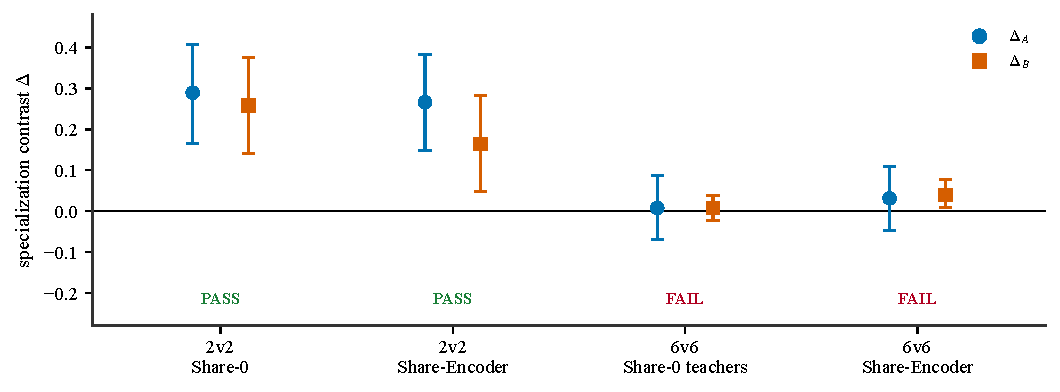
\includegraphics[width=0.94\textwidth]
        {plots/combined/fig_specialization_scaling_2v2_6v6.pdf}
    \caption{Closed-loop specialization across team sizes, under one criterion.
    At $2$-vs-$2$, both the zero-sharing reference and the shared-encoder
    controller satisfy the criterion, and the $48.0\%$ parameter reduction is
    obtained without detectable paired loss. At $6$-vs-$6$, \emph{neither} the
    zero-sharing reference nor the shared-encoder controller satisfies it. The
    failure therefore does not localize to compression: the uncompressed
    specialists do not exhibit complementary payoff specialization either.
    Error bars denote $95\%$ paired bootstrap confidence intervals; the two
    $6$-vs-$6$ evaluations use disjoint seed blocks and are not paired with each
    other.}
    \label{fig:scale-specialization}
\end{figure*}

% OPTIONAL companion (built, available at plots/combined/):
%   fig_cross_scale_2v2_6v6.pdf
%     three panels -- (a) demand certified at both scales, (b) ~99% of teacher
%     branch divergence retained at both scales under an identical 48.0% cut,
%     (c) the same four-condition payoff comparison as above.
%     Use if you want demand + fidelity + payoff carried in a single float;
%     it overlaps this figure's panel (c), so include one or the other.
%   fig_6v6_payoff_share0_vs_encoder.pdf
%     absolute 6v6 win-rate cells, teachers vs. shared-encoder student.
%     Useful if a reviewer asks whether the 6v6 policies are simply weak --
%     they are not; every cell lies between 0.836 and 0.992.

The comparison across scales is deliberately based on specialization
contrasts rather than raw win rates. Absolute task difficulty changes with
team size, so a direct comparison of win-rate magnitudes would confound
strategic specialization with changes in the underlying game. In contrast,
$\Delta_A$ and $\Delta_B$ ask the same question at both scales: whether each
policy retains a relative advantage in the opponent regime for which it was
trained.

%----------------------------------------------------------------------
\subsection{Deployment robustness after strategy preservation}
\label{sec:exp-robustness}
%----------------------------------------------------------------------

The preceding experiments separate two questions: whether strategic content
survives architectural sharing, and whether the preserved controller remains
stable under imperfect deployment conditions. We examine the latter using the
$2$-vs-$2$ Share-Encoder controller, because it is the strongest sharing level
that preserves specialization without detectable paired loss.

Localization perturbations preserve the specialization criterion at every
tested level,
\[
    \sigma\in\{0.03,0.06,0.12\}.
\]
Motion uncertainty produces a different response: specialization fails at all
tested levels through Regime~B. Control delay exhibits a clearer dose response,
with the Regime-A contrast decreasing from approximately $0.180$ under nominal
execution to $0.109$ with one tick of delay and $0.031$ with two ticks.

These perturbation results therefore complement, rather than redefine, the
scaling analysis. The $2$-vs-$2$ sharing experiment identifies where strategic
content is retained, the $6$-vs-$6$ experiment tests whether that content is
recoverable at larger coordination scale, and the perturbation experiments
characterize how the preserved controller responds to deployment uncertainty.
Together, the results distinguish architectural preservation, scaling, and
deployment robustness as separate but connected aspects of shared multi-robot
strategy representation.
